\documentclass{beamer}
\usepackage{beamerthemesplit}
\usepackage{graphics}
\logo{
\includegraphics[height=1cm]{psi_logo_white.png}}
\usetheme{Pittsburgh}
\usecolortheme{dove}
\beamertemplatenavigationsymbolsempty
\setbeamertemplate{footline}[frame number]
\definecolor{myback}{RGB}{175,238,238}
\setbeamercolor{structure}{bg=myback}
\usepackage[T1]{fontenc}
\newcommand{\changefont}[3] {
 \fontfamily{#1} \fontseries{#2} \fontshape{#3} \selectfont}

\title{NeXus Code Camp 2012}
\author{Mark K\"onnecke }
\institute{Paul Scherrer Institute\\Switzerland }
\date{\today} 

\begin{document}

\begin{frame}
\titlepage
\end{frame}

\begin{frame}
\frametitle{General Topics}
\begin{itemize}
\item Finalize CIF coordinate Issue
\item Change of documentation form docbook to Sphinx
\item Cleanup trac tickets
\item Develop a materials definition
\item Do we need specials for timed data?
\item DECTRIS (again) 
\item Review OO-NeXus status?
\end{itemize}
\end{frame}

\begin{frame}
\frametitle{Technical Topics}
\begin{itemize}
\item PyTree API Tests
\item Automatisation and documentation of the NeXus release process
\begin{itemize}
\item Continuous integration
\item Write more or proper unit tests
\end{itemize}
\item CMake versus autoconf
\item NXdict replacement design
\end{itemize}
\end{frame}

\begin{frame} \frametitle{CIF Coordinate Issue }
\begin{itemize}
\item Decided: extend NeXus to allow full mapping from CBF to NeXus
\item Information to encode:
\begin{description}
\item[type] rotation or translation: DONE! transformation\_type attribute
\item[direction] vector around which to rotate or along which to translate: DONE! attribute
\item[value] The angle of rotation or the length of translation, DONE!
\item[dependency] The order of operations to place a component, to be discussed!
\end{description}
\end{itemize}
\end{frame}


\begin{frame} \frametitle{Expressing Axis Dependency in NeXus}
\begin{itemize}
\item Implied: use existing NeXus coordinate system
\item dependson attribute pointing to depending axis
\item transform field in base classes which becomes a comma separated list of 
 the path to the transformations required to position this component
\item Create a special container to hold axis dependencies, NXdependency, to 
 collect the dependencies in one place for easy access. This is what CIF does
\end{itemize}
\end{frame}

\begin{frame} \frametitle{Dependons Option}
\begin{tabbing}
\hspace*{1cm} \= \hspace*{1cm} \= \hspace*{1cm} \= \hspace*{1cm} \= \hspace*{1cm} \= \hspace*{1cm}\= \kill
\>sample,NXsample\\
\> \>rotation\_angle\\
\> \>chi (dependson rotation\_angle)\\
\> \>phi (dependson phi)\\
\end{tabbing}
\end{frame}

\begin{frame} \frametitle{Transform Option}
\begin{tabbing}
\hspace*{1cm} \= \hspace*{1cm} \= \hspace*{1cm} \= \hspace*{1cm} \= \hspace*{1cm} \= \hspace*{1cm}\= \kill
\>sample,NXsample\\
\> \>rotation\_angle\\
\> \>chi \\
\> \>phi \\
\> \>transform = rotation\_angle,chi,phi \\
\end{tabbing}
\end{frame}


\begin{frame} \frametitle{Separate Group Option}
\begin{tabbing}
\hspace*{1cm} \= \hspace*{1cm} \= \hspace*{1cm} \= \hspace*{1cm} \= \hspace*{1cm} \= \hspace*{1cm}\= \kill
\>sample,NXsample\\
\> \>rotation\_angle\\
\> \>chi \\
\> \>phi \\
\>dependency,NXdependency\\
\> \>sample/chi = \\
\> \> \>sample/rotation\_angle\\
\> \>sample/phi =\\
\> \> \> sample/chi\\
\> \>instrument/detector/x\_translation = \\
\> \> \>instrument/detector/distance\\
\> \>instrument/detector/distance = \\
\> \> \>instrument/detector/polar\_angle\\
\end{tabbing}
\end{frame}


\begin{frame} \frametitle{Change Documentation from Docbook to Sphinx}
\begin{itemize}
\item Current documentation in Docbook
\item Only experts can write docbook
\item Sphinx is restructed Text which is easy to write
\item RST converts into many formats including html and pdf
\item Issues:
\begin{itemize}
\item Do we like the look of Sphinx?
\item How can we convert automatically?
\item Integration with CMake
\end{itemize}
\end{itemize}
\end{frame}

\begin{frame} \frametitle{NXdict replacement Design}
\begin{itemize}
\item Current NXDict
\begin{itemize}
\item File format to describe items in a NeXus file
\item API to generate structure and read data from NeXus file
\item Found little (or no) use outside of PSI
\end{itemize}
\end{itemize}
\end{frame}



\begin{frame}[fragile]
 \frametitle{NXDict file format }
\begin{semiverbatim}            
##NXDICT-1.0
etitle=/entry,NXentry/SDS title -type NX_CHAR -rank 1
instrument=/entry,NXentry/SDS instrument -type NX_CHAR -rank 1
estart=/entry,NXentry/SDS start_time -type DFNT_CHAR -rank 1 
eend=/entry,NXentry/SDS end_time -type DFNT_CHAR -rank 1 
edef=/entry,NXentry/SDS definition -type DFNT_CHAR -rank 1 

table=table2
var=sdw
units=mm
tablevar=/entry,NXentry/$(table),NXCollection/SDS $(var) -rank 1 -dim {-1} -attr {units,$(units)}
tabledet=/entry,NXentry/$(table),NXCollection/SDS detector -type NX_CHAR -rank 1
tablequip=/entry,NXentry/$(table),NXCollection/SDS equipment -type NX_CHAR -rank 1
tabletext=/entry,NXentry/$(table),NXCollection/SDS $(var) -rank 1 -dim {-1} -type NX_CHAR
	
\end{semiverbatim}
\end{frame}


\begin{frame}[fragile]
 \frametitle{NXDict dictionary Maintenance API }
\begin{semiverbatim}
NXstatus NXDinitfromfile(char *filename, NXdict * pDict);
NXstatus NXDclose(NXdict handle, char *filename);

NXstatus NXDadd(NXdict handle, char *alias, char *DefString);
NXstatus NXDget(NXdict handle, char *alias, char *pBuffer, int iBufLen);
NXstatus NXDupdate(NXdict handle, char *alias, char *pNewVal);
NXstatus NXDtextreplace(NXdict handle, char *pDefString, char *pBuffer,
                        int iBuflen);
	
\end{semiverbatim}
\end{frame}



\begin{frame}[fragile]
 \frametitle{NXDict dictionary Data Transfer API }
\begin{semiverbatim}
NXstatus NXDputalias(NXhandle file, NXdict dict, char *alias, void *pData);
NXstatus NXDputdef(NXhandle file, NXdict dict, char *pDefString,
                   void *pData);

NXstatus NXDgetalias(NXhandle file, NXdict dict, char *alias, void *pData);
NXstatus NXDgetdef(NXhandle file, NXdict dict, char *pDefString,
                   void *pData);
NXstatus NXDdefget(NXdict handle, char *pKey, char *pBuffer, int iBufLen);

NXstatus NXDaliaslink(NXhandle file, NXdict dict,
                      char *pAlias1, char *pAlias2);
NXstatus NXDdeflink(NXhandle file, NXdict dict, char *pDef1, char *pDef2);

NXstatus NXDopenalias(NXhandle file, NXdict dict, char *alias);
NXstatus NXDopendef(NXhandle file, NXdict dict, char *pDefString);

\end{semiverbatim}
\end{frame}


\begin{frame} \frametitle{Future NXdict }
\begin{itemize}
\item Base on NXDL?
\item Competition to CDF?
\item Is there still a need? 
\end{itemize}
\end{frame}

\begin{frame} \frametitle{Timed Data}
\begin{itemize}
\item Event mode data
\item On the fly scans at synchrotrons
\item Groups of parameters being collected on possibly 
   different sampling intervalls
\item Group of NXlogs? This then is the data!
\item Or scan like: each parameter can become a NXlog in its 
  place in the hierarchy, links in NXdata? 
\item Other ideas?
\item Or no problem at all? 
\item I want a clear statement how this is done in NeXus!
\end{itemize}
\end{frame}



\begin{frame} \frametitle{Materials Definition}
\begin{itemize}
\item How to describe complex materials: samples, sensors, multi layers etc? 
\item Chemical formula: steal CIF conventions? 
\item Some research required
\end{itemize}
\end{frame}

\begin{frame} \frametitle{NeXus Release Process}
\begin{itemize}
\item Problem: only Freddie knows how to make a NeXus release
\item Solution 1: document and have privileges
\item Solution 2: automatise (but do not get lost in tooling....)
\end{itemize}
\end{frame}


\begin{frame} \frametitle{Prioritise!}
\end{frame}














\begin{frame} \frametitle{Transformation Matrices}
\begin{math}
T = \left( \begin{array}{cccc}
1 & 0 & 0 & x\\
0 & 1 & 0 & y\\
0 & 0 & 1 & z\\
0 & 0 & 0 & 1\\
\end{array} \right)
\end{math}

\begin{math}
\onslide+<2-> 
R = \left( \begin{array}{cccc}
r11 & r12 & r13 & 0\\
r21 & r22 & r23 & 0\\
r31 & r32 & r33 & 0\\
0 & 0 & 0 & 1\\
\end{array} \right)
\end{math}

\end{frame}

\begin{frame} \frametitle{Combining Transformations}
\begin{figure}[!ht]
\resizebox{7cm}{5cm}{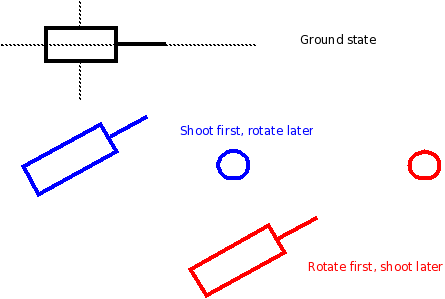
\includegraphics[width=0.75\textwidth]{rotcombi.png}}\end{figure}
\end{frame}

\begin{frame} \frametitle{Some Properties}
\begin{itemize}
\item Transformations can be combined by matrix multiplications
\item Individual matrices can be derived by looking at the situation when everything else is 0
\item Absolute positions can be obtained by multiplying the resulting matrix with its transpose
\item Defines new coordinate systems at components
\item CIF contains a duplication: vector, offset scheme 
\end{itemize}
\end{frame}

\begin{frame} \frametitle{What Use Is This?}
\begin{itemize}
\item Allows to calculate absolute positions of components in the laboratory coordinate systems
\item Can directly convert from a detector coordinate system to  
 vectors in Lab coordinate system
\item Calculate things like impact of primary beam on detector, SAS
\item Allows arbitray axis to be expressed
\item Intuitively describe an instrument with angles and translations and still be able
 to recover absolute coordinates
\end{itemize}
\end{frame}


\begin{frame} \frametitle{NeXus Axis Mapped}
\begin{itemize}
\item rotation\_angle, polar\_angle, rotate 0 1 0
\item azimuthal\_angle, rotate 0 0 1
\item distance, translate 0 0  1
\item chi, rotate 0 0 1
\item phi rotate, 0 1 0
\item NeXus polar coordinate system: rotate azimuthal\_angle, rotate polar\_angle, 
 translate by distance
\end{itemize}
\end{frame}

\begin{frame} \frametitle{CIF Dependency Table}
\begin{tabular}{llllll}
axis-id &type &equipment&dependson &vector & offset\\
gonio\_phi &rotation& goniometer & . &1,0,0,& ...\\
det\_z&translation&detector& .& 0,0,-1& 0 0 0\\
det\_y&translation&detector&det\_z&0,1,0&0,0,0\\
det\_x&translation&detector&det\_y&1,0,0&0,0,0\\
\end{tabular}
\end{frame}



\begin{frame} \frametitle{DECTRIS Again }
\begin{figure}[!ht]
\resizebox{7cm}{5cm}{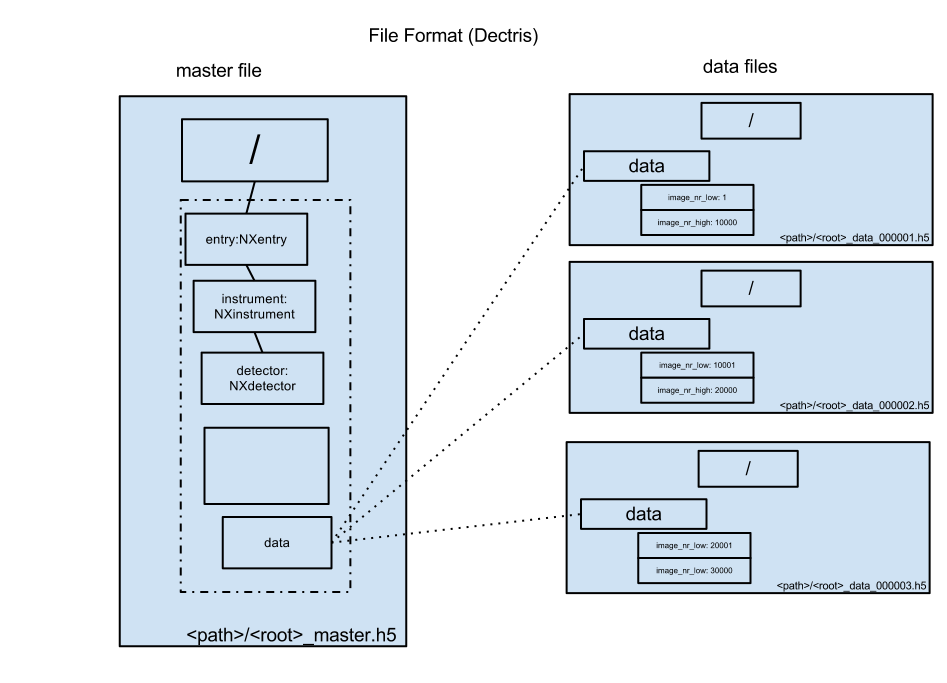
\includegraphics[width=0.75\textwidth]{HDF5-FileOrganisation.png}}\end{figure}
\end{frame}
\begin{frame}
\frametitle{Rationale}
\begin{itemize}
\item DECTRIS has a problem:
\begin{itemize}
\item Detector outputs 5-10 GB/sec
\item The deliver the detector and the computer going with it
\item They cannot ask their customers to provide the appropriate hardware for such 
 a detector: parallel file system etc.
\item Must compress and write the file on one computer
\item Compression has to be parallel as CPU intensive
\end{itemize}
\item File structure a workaround for HDF-5 not allowing sections of datsets in different 
 files
\item Sidenote: LZ4 or snappy compression; up to ~ 450MB/sec on write
\end{itemize}
\end{frame}


\begin{frame}
\frametitle{Upcoming DECTRIS Meeting with Community}
\begin{itemize}
\item DECTRIS aims at meeting customers in october
\item How far can we compromise?
\item Anyone from the NeXus community who wishes to join?
\end{itemize}
\end{frame}




\end{document}





\begin{frame} \frametitle{}
\begin{itemize}
\item 
\item 
\item 
\end{itemize}
\end{frame}

\begin{frame} \frametitle{Easy Plotting}
\begin{tabbing}
\hspace*{1cm} \= \hspace*{1cm} \= \hspace*{1cm} \= \hspace*{1cm} \= \hspace*{1cm} \= \hspace*{1cm}\= \kill
\>data,NXdata\\
\> \>data[nx,ny]\\
\> \> \>@signal=1 \\
\> \>x[nx]\\
\> \> \>@axis=1\\
\> \>y[ny]\\
\> \> \>@axis=2\\
\end{tabbing}
\end{frame}


\begin{frame} \frametitle{Careful Data Analysis}
\begin{tabbing}
\hspace*{1cm} \= \hspace*{1cm} \= \hspace*{1cm} \= \hspace*{1cm} \= \hspace*{1cm} \= \hspace*{1cm}\= \kill
\>data,NXdata\\
\> \>data[nx,ny]\\
\> \> \>@signal=1 \\
\> \>x[nx,ny]\\
\> \>y[nx,ny]\\
\end{tabbing}
\end{frame}

\begin{frame} \frametitle{Tobias Suggestion}
\begin{tabbing}
\hspace*{1cm} \= \hspace*{1cm} \= \hspace*{1cm} \= \hspace*{1cm} \= \hspace*{1cm} \= \hspace*{1cm}\= \kill
\>data,NXdata\\
\> \>data[nx,ny]\\
\> \> \>@signal=1 \\
\> \>x[nx,ny]\\
\> \> \>@axis=1,2\\
\> \> \>@label=1\\
\> \>y[nx,ny]\\
\> \> \>@axis=1,2\\
\> \> \>@label=2\\
\end{tabbing}
\end{frame}

\begin{frame} \frametitle{Marks Suggestion}
\begin{tabbing}
\hspace*{1cm} \= \hspace*{1cm} \= \hspace*{1cm} \= \hspace*{1cm} \= \hspace*{1cm} \= \hspace*{1cm}\= \kill
\>data,NXdata\\
\> \>data[nx,ny]\\
\> \> \>@signal=1 \\
\> \> \>@axes=x,y \\
\> \> \>@axesvalue=x\_scan,y\_scan \\
\> \>x[nx]\\
\> \> \>@axis=1\\
\> \>y[ny]\\
\> \> \>@axis=2\\
\> \>x\_scan[nx,ny]\\
\> \>y\_scan[nx,ny]\\
\end{tabbing}
\end{frame}

\begin{frame} \frametitle{More Suggestions?}
\begin{tabbing}
\hspace*{1cm} \= \hspace*{1cm} \= \hspace*{1cm} \= \hspace*{1cm} \= \hspace*{1cm} \= \hspace*{1cm}\= \kill
\>data,NXdata\\
\> \>data[nx,ny]\\
\> \> \>@signal=1 \\
\end{tabbing}
\end{frame}

\begin{frame}
\frametitle{NXdetector Extensions for Dectris}
\begin{itemize}
\item Dectris (Eiger, Pilatus, Mythen) going HDF-5 with NeXus conventions
\item Additions to NXdetector for this kind of detector
\item Programming model:
\begin{itemize}
\item Dectris writes HDF-5 file with NXdetector
\item Local DAQ-system adds beamline metadata   
\end{itemize}
\end{itemize}
\end{frame}








\begin{frame} \frametitle{NeXus Simple Coordinate System }
\begin{figure}[!ht]
\resizebox{7cm}{5cm}{\includegraphics[width=0.75\textwidth]{polplane.png}}\end{figure}
\end{frame}

\begin{frame}
\frametitle{The Predicament of the Traveling Scientist}
\begin{itemize}
\item<1->A different data format wherever she goes
\item<2->Spends lots of time converting formats or writing readers
\item<3->Waits even longer to load data from inefficient data formats
\item<4->DA requires N files in different  formats, notes, local knowledge 
\item<5->Cannot read her collaborators data
\item<6->Has to keep extra information in yet another form
\end{itemize}
\end{frame}

